\documentclass[tikz,border=0pt]{standalone}
\usepackage[T1]{fontenc}
\usepackage{helvet}
\usepackage{amsmath,amssymb}
\usepackage{fix-cm}
\renewcommand{\familydefault}{\sfdefault}
\usetikzlibrary{arrows.meta,calc,decorations.pathreplacing}
\pdfinfoomitdate=1
\pdftrailerid{}
\definecolor{ink}{HTML}{000000}
\definecolor{blue}{HTML}{3B86FF}
\definecolor{green}{HTML}{00A14B}
\definecolor{orange}{HTML}{FC4D30}
\definecolor{gold}{HTML}{FFC943}
\definecolor{purple}{HTML}{A93BFF}
\definecolor{muted}{HTML}{7F7F7F}
\definecolor{neutral}{HTML}{F1F2F2}
\definecolor{palegold}{HTML}{FFDD92}
\definecolor{rule}{HTML}{D9D9D9}
\newcommand{\meter}[3]{%
 \begin{scope}[shift={(#1,#2)}]
  \draw[ink,fill=#3,rounded corners=1pt,line width=.65pt] (-.24,-.22) rectangle (.24,.22);
  \draw[ink,line width=.5pt] (-.16,-.075) arc[start angle=155,end angle=25,radius=.18];
  \draw[ink,line width=.6pt,-{Stealth[length=1.1mm]}] (0,-.075)--(.105,.12);
 \end{scope}}
% BEGIN REPRODUCIBLE INPUT SAMPLES
\def\MGsamples{%
0/0.38764364216757924,
1/0.40615720119773024,
2/0.4463915793931561,
3/0.50817760747773955,
4/0.58519930772035222,
5/0.66729722191215257,
6/0.74505917630328977,
7/0.81247106892069176,
8/0.86689167975861015,
9/0.90794272424834443,
10/0.93646540885372742,
11/0.95384551205609003,
12/0.96164928946538053,
13/0.96145965892131113,
14/0.95483835566866182,
15/0.94337955489436875,
16/0.92883927830309254,
17/0.91332532592686089,
18/0.89951558218351002,
19/0.89078554189727899,
20/0.89095726413519727,
21/0.90338045822842616,
22/0.92953357891376454,
23/0.9677434882368493,
24/1.0125195980807131,
25/1.0556636937755013,
26/1.0899536247702448,
27/1.1124773138628472,
28/1.1245540784425698,
29/1.1296093315051245,
30/1.1313801870848861,
31/1.1330425872159817,
32/1.1369007867325696,
33/1.1442890513970521,
34/1.1555508925368432,
35/1.170110017891405,
36/1.1866765942143243,
37/1.2035328744395946,
38/1.2186670957242458,
39/1.2294555068812938,
40/1.2319902989980167,
41/1.2212902864412309,
42/1.1941225089277439,
43/1.1523633996860949,
44/1.1018827430328695,
45/1.0486944298581569,
46/0.99693923450855537,
47/0.94879210762634925,
48/0.90491896258764248,
49/0.86492947417662602,
50/0.82778481397601622,
51/0.79220242048611667,
52/0.75704405557601384,
53/0.7216094655334595,
54/0.6857514907575557,
55/0.64980806555053328,
56/0.61445972220822676,
57/0.58067014972080067,
58/0.54981399695307542,
59/0.52397249622742481,
60/0.50621224921814256,
61/0.50052209412064663,
62/0.51103818398539114,
63/0.5403324767428378,
64/0.58752107115320995,
65/0.64802630677037432,
66/0.71550135682131888,
67/0.78409808386961188,
68/0.84951718853604397,
69/0.90894935129625243,
70/0.96064650870025381,
71/1.0035822016633544,
72/1.0372911621199843,
73/1.0618022847988742,
74/1.077578297308732,
75/1.0854505724927239,
76/1.0865914236887313,
77/1.0825635706693835,
78/1.0754379232179192,
79/1.0678998632935517,
80/1.0631934943792889,
81/1.0647118795606736,
82/1.0751718923021236,
83/1.0955892045147246,
84/1.1242694426333708,
85/1.1559990642195355,
86/1.1824875215959869,
87/1.1955003607996595,
88/1.1910444327682601,
89/1.1705040957716952,
90/1.1384031218268023,
91/1.099827075953888,
92/1.0591197193008617,
93/1.0195882388041739,
94/0.98359606042482139,
95/0.95267073565665794,
96/0.92747747821991278,
97/0.90765178270382629,
98/0.89161365530325176,
99/0.87659488486027026,
100/0.85910878244251354,
101/0.83595370602281049,
102/0.80556188398914175,
103/0.76894649106923407,
104/0.72932359418630777,
105/0.69072770482022727,
106/0.65697202025912493,
107/0.63144601534941625,
108/0.61720590627165262,
109/0.61676268788334365,
110/0.63139102242782441,
111/0.66035221677358302,
112/0.70079243403788782,
113/0.74863376221030531,
114/0.79987082286849076,
115/0.85147674986199073,
116/0.90167664022541871,
117/0.94978294133316643,
118/0.99575550277720715,
119/1.039487550085922,
120/1.0800242032092209,
121/1.1154457556509538,
122/1.1438086790634479,
123/1.1642406236883278,
124/1.1772719164838901,
125/1.1845739187475659,
126/1.1885753029378479,
127/1.1920955818683334,
128/1.1979054146325014,
129/1.208135250616813,
130/1.2235872514710875,
131/1.2431098048034033,
132/1.2632840394997009,
133/1.2788303961798322,
134/1.2840136891526057,
135/1.2745306350622621,
136/1.2487705408842895,
137/1.207961546433383,
138/1.1555341435328266,
139/1.0960073570071789,
140/1.0337403272711418,
141/0.97212990235904573,
142/0.91342707821539926,
143/0.85887075146313485,
144/0.8088550600241502,
145/0.76305303745842412,
146/0.72056534976013464,
147/0.68019953050383941,
148/0.64089460212871052,
149/0.60214263246823174,
150/0.56418562132730077,
151/0.52790852833879554,
152/0.49459990816499949,
153/0.46584539734016805,
154/0.44369378827434613,
155/0.43105017534770285,
156/0.43201156538945434,
157/0.45141934884143836,
158/0.49265550239771172,
159/0.55425122683235384,
160/0.6289130993767168,
161/0.70700368574501027,
162/0.78075861028325722,
163/0.84572140140270746,
164/0.90002209297046842,
165/0.94323544164717388,
166/0.97560954631743935,
167/0.99772720614744248,
168/1.0104241114534918,
169/1.0147862132104319,
170/1.0121409882487495,
171/1.0040511479563912,
172/0.9923585595990011,
173/0.97931365160998429,
174/0.96776503898988331,
175/0.96124069025605208,
176/0.96356480518617138,
177/0.97775614564111657,
178/1.0045571629411014,
179/1.041223367253084,
180/1.0811295768379747,
181/1.1154915892708783,
182/1.137401221470691,
183/1.1447871941686614,
184/1.1398538758060661,
185/1.1267762644178936,
186/1.1099066118657155,
187/1.0929604169477352,
188/1.0787786782920614,
189/1.0692765302821474,
190/1.0653889530026306,
191/1.0669797628507403,
192/1.0727728179699243,
193/1.0803751371861599,
194/1.0863732283199725,
195/1.0864626817606129,
196/1.0759887577071325,
197/1.0517628177745251,
198/1.0145476590577551,
199/0.96910458477775108,
200/0.92139423414216393
}
% END REPRODUCIBLE INPUT SAMPLES
% BEGIN ILLUSTRATIVE OUTPUT COMPARISONS
\def\OutputSamples{%
0/0.66977623801848196/0.66977623801848196,
1/0.65583834699898524/0.65583834699898524,
2/0.65000000000000002/0.65000000000000002,
3/0.65570821348824393/0.65570821348824393,
4/0.67676329766029131/0.67676329766029131,
5/0.71528022631080934/0.71528022631080934,
6/0.76912404276983359/0.76912404276983359,
7/0.83169849724428291/0.83169849724428291,
8/0.8949904948323153/0.8949904948323153,
9/0.95274803110852435/0.95274803110852435,
10/1.0014855539525096/1.0014855539525096,
11/1.0399454084916389/1.0399454084916389,
12/1.0682356131074942/1.0682356131074942,
13/1.0871723806939197/1.0871723806939197,
14/1.0978824876184476/1.0978824876184476,
15/1.1015922273716672/1.1015922273716672,
16/1.0995351159228774/1.0995351159228774,
17/1.0929408398228837/1.0929408398228837,
18/1.0830921118139831/1.0830921118139831,
19/1.0714444542623636/1.0714444542623636,
20/1.0597950394412368/1.0597950394412368,
21/1.0504510904083475/1.0504510904083475,
22/1.0462461469620945/1.0462461469620945,
23/1.0501358303320272/1.0501358303320272,
24/1.0642615751946756/1.0642615751946756,
25/1.0888378026007748/1.0888378026007748,
26/1.1213038892154032/1.1213038892154032,
27/1.1562216506585439/1.1562216506585439,
28/1.1870343641074581/1.1870343641074581,
29/1.2092817665445925/1.2092817665445925,
30/1.222229851432953/1.222229851432953,
31/1.227867152774647/1.227867152774647,
32/1.2291674421271146/1.2291674421271146,
33/1.2289787278798376/1.2289787278798376,
34/1.2295654948310251/1.2295654948310251,
35/1.2324662025458917/1.2324662025458917,
36/1.2384518781359752/1.2384518781359752,
37/1.2475295504354036/1.2475295504354036,
38/1.2590201363838061/1.2590201363838061,
39/1.2717325108342532/1.2717325108342532,
40/1.2841513815958843/1.0341513815958843,
41/1.2944258832271107/1.0444258832271107,
42/1.3/1.05,
43/1.2972893793140956/1.0472893793140956,
44/1.2827230711277813/1.0327230711277813,
45/1.2555554306963459/1.0055554306963459,
46/1.2190947599542541/0.96909475995425409,
47/1.1783304237499095/0.92833042374990948,
48/1.1373798984643977/0.88737989846439769,
49/1.0987589302529908/0.84875893025299076,
50/1.0636007699233276/0.81360076992332764,
51/1.0320161900230342/0.78201619002303413,
52/1.003410668599833/0.75341066859983297,
53/0.97678779435755847/0.72678779435755847,
54/0.95106292556625704/0.70106292556625704,
55/0.92535671573014966/0.67535671573014966,
56/0.89919767820338958/0.64919767820338958,
57/0.87257617059342529/0.62257617059342529,
58/0.84586978833581328/0.59586978833581328,
59/0.81974651704266821/0.56974651704266821,
60/0.79517003835446576/0.54517003835446576,
61/0.77356361336573332/0.52356361336573332,
62/0.75706173526919385/0.50706173526919385,
63/0.74861943571634515/0.49861943571634515,
64/0.75164585475626322/0.50164585475626322,
65/0.76887296140832861/0.51887296140832861,
66/0.80070632280793097/0.55070632280793097,
67/0.84440386155828351/0.59440386155828351,
68/0.89516539348988355/0.64516539348988355,
69/0.94812562205391537/0.69812562205391537,
70/0.9995863951860986/0.7495863951860986,
71/1.0471606683483841/0.79716066834838406,
72/1.0894087565852233/0.83940875658522329,
73/1.1254667574525972/0.87546675745259717,
74/1.1548438517320672/0.90484385173206727,
75/1.1773630619006041/0.92736306190060414,
76/1.1931558383132139/0.94315583831321403,
77/1.2026513891771677/0.95265138917716785,
78/1.2065636284432546/0.9565636284432546,
79/1.2059120500497733/0.9559120500497732,
80/1.2020980711797287/0.95209807117972867,
81/1.1970045085016328/0.94700450850163276,
82/1.1930163813446999/0.94301638134469978,
83/1.1928050565682899/0.94280505656828983,
84/1.1987580758890684/0.94875807588906835,
85/1.2121541225528101/0.96215412255281019,
86/1.2323128147621738/0.9823128147621738,
87/1.2558850003991355/1.0058850003991355,
88/1.2768795463732556/1.0268795463732556,
89/1.2885758656329034/1.0385758656329034,
90/1.286810527211093/1.036810527211093,
91/1.2716391491751646/1.0216391491751646,
92/1.2461340468576956/0.99613404685769569,
93/1.2142842491090655/0.96428424910906552,
94/1.1796905736214252/0.92969057362142515,
95/1.1451571732032788/0.89515717320327881,
96/1.1127170444927594/0.86271704449275943,
97/1.0837457509770698/0.83374575097706993,
98/1.0590011431865622/0.80900114318656224,
99/1.0385418411394005/0.78854184113940051,
100/1.0215733175101545/0.77157331751015445
}
% END ILLUSTRATIVE OUTPUT COMPARISONS
\begin{document}
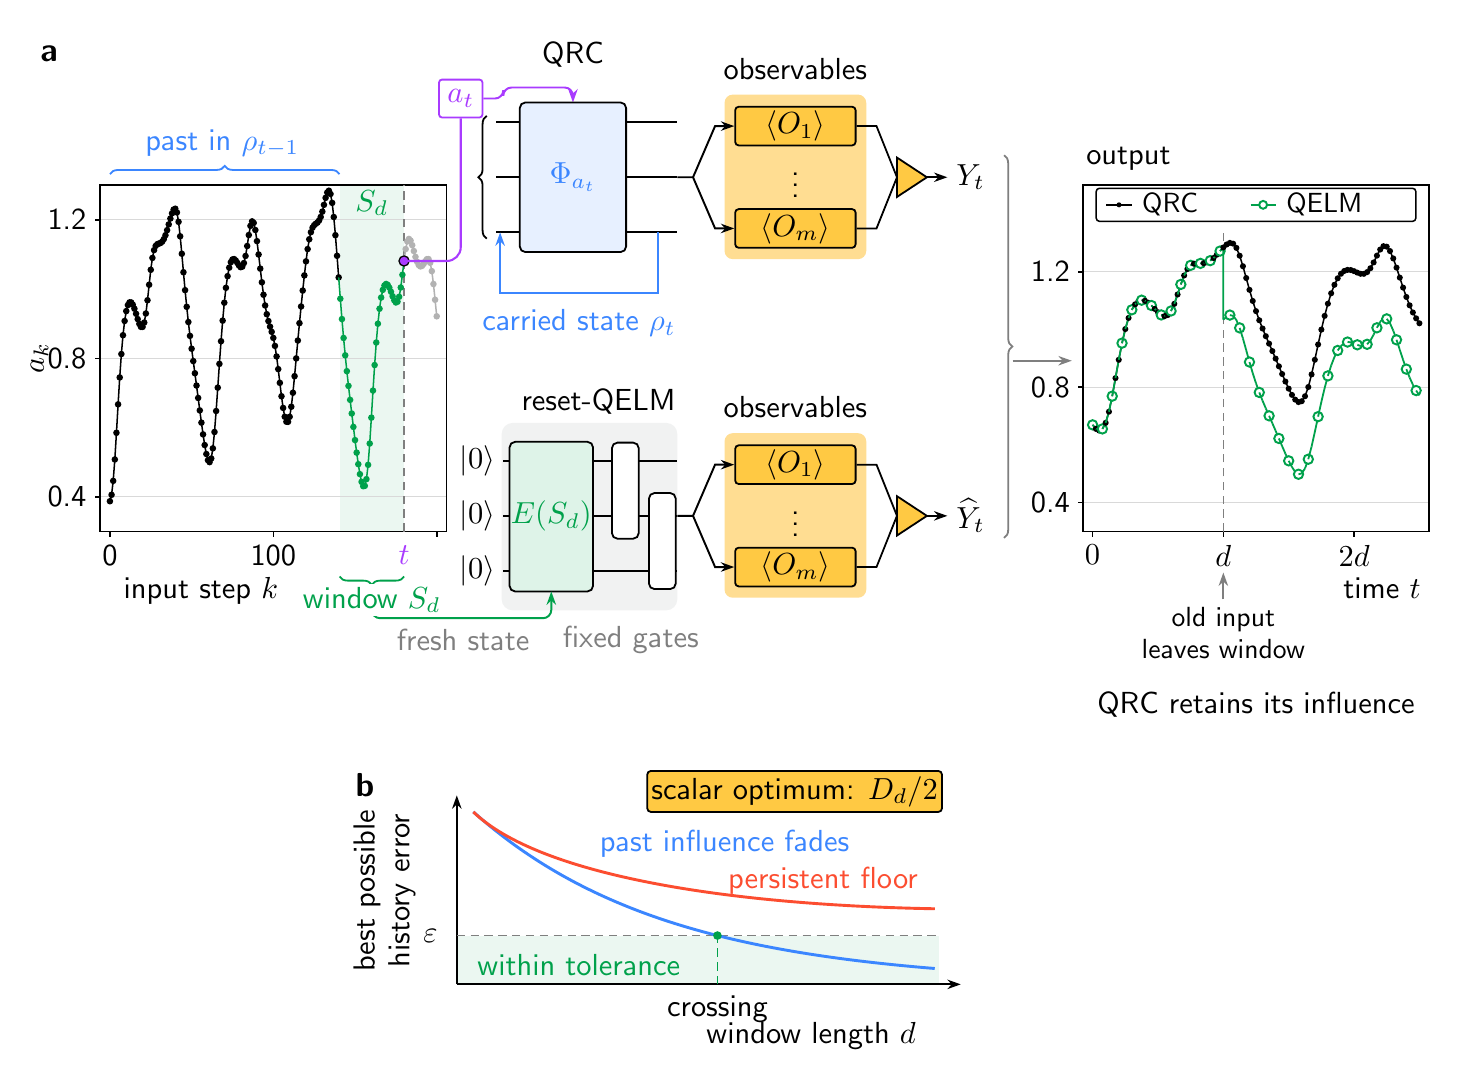
\begin{tikzpicture}[x=1cm,y=1cm,line width=.65pt,text=ink,
 font=\fontsize{11}{12.5}\selectfont,
 every node/.style={inner sep=1.5pt},
 flow/.style={-{Stealth[length=1.7mm,width=1.2mm]},line width=.7pt},
 letter/.style={anchor=west,font=\bfseries\fontsize{12}{13}\selectfont},
 feature/.style={draw=ink,fill=gold,rounded corners=1.3pt,minimum width=1.53cm,
                  minimum height=.48cm,line width=.65pt}]
\useasboundingbox (0,0) rectangle (17.9197,13.0);
\fill[white] (0,0) rectangle (17.9197,13.0);

% a: two architectures feed one shared prediction-comparison column.
\node[letter] at (.10,12.67) {a};
% One shared square input plot, centered between the two model lanes.
% Only 0--180 are available at t; grey values 181--200 are display context.
\fill[green!8] ({.92+4.4*146.5/212},6.60) rectangle ({.92+4.4*186/212},11.00);
\foreach \val in {0.4,0.8,1.2}{
 \pgfmathsetmacro{\yy}{6.60+4.4*(\val-.3)}
 \draw[rule,line width=.35pt] (.92,\yy)--(5.32,\yy);
 \draw[ink,line width=.55pt] (.86,\yy)--(.92,\yy);
 \node[anchor=east] at (.81,\yy) {\val};
}
\draw[ink,line width=.6pt] (.92,6.60) rectangle (5.32,11.00);
\foreach \kk in {0,100}{
 \pgfmathsetmacro{\xx}{.92+4.4*(\kk+6)/212}
 \draw[ink,line width=.55pt] (\xx,6.60)--(\xx,6.53);
 \node[anchor=north] at (\xx,6.49) {\kk};
}
\draw[ink,line width=.55pt] ({.92+4.4*206/212},6.60)--({.92+4.4*206/212},6.53);
\node[anchor=north,text=purple] at ({.92+4.4*186/212},6.49) {$t$};
\node[rotate=90] at (.15,8.80) {$a_k$};
\node[anchor=north] at (2.20,6.08) {input step $k$};
\draw[muted,densely dashed,line width=.55pt] ({.92+4.4*186/212},6.60)--({.92+4.4*186/212},11.00);
\begin{scope}[shift={(1.04452830188679,5.28)},x=.0207547169811321cm,y=4.4cm]
 \foreach \kk/\val [remember=\kk as \pk (initially 0),
                    remember=\val as \pv (initially 0)] in \MGsamples{
  \def\tracecolor{ink}
  \ifnum\kk>140 \def\tracecolor{green}\fi
  \ifnum\kk>180 \def\tracecolor{muted!60}\fi
  \ifnum\kk>0 \draw[\tracecolor,line width=.55pt] (\pk,\pv)--(\kk,\val);\fi
  \node[fill=\tracecolor,circle,inner sep=.84pt] at (\kk,\val) {};
  \ifnum\kk=180 \coordinate (currentinput) at (\kk,\val);\fi
 }
\end{scope}
\node[draw=ink,fill=purple,circle,line width=.45pt,inner sep=1.30pt] at (currentinput) {};
\node[text=green,fill=green!8,inner sep=.5pt] at (4.37,10.77) {$S_d$};

% The old-input brace identifies information carried in the QRC state.
% It is not a second input wire or a claim that all history is stored losslessly.
\draw[blue,decorate,decoration={brace,amplitude=3pt}]
 ({.92+4.4*6/212},11.14)--({.92+4.4*146.5/212},11.14);
\node[text=blue] at (2.47,11.53) {past in $\rho_{t-1}$};

% Only the current scalar enters each general QRC channel update.
% Its leader starts at the actual ordinate and stays clear of quantum wires.
\node[draw=purple,rounded corners=1pt,text=purple,fill=white,
 minimum width=.55cm,minimum height=.48cm] (inputnode) at (5.50,12.10) {$a_t$};
\draw[purple,line width=.75pt,rounded corners=5pt]
 (currentinput)--(5.50,0 |- currentinput)--(inputnode.south);
\draw[flow,purple,rounded corners=3pt] (inputnode.east)--(6.04,12.10)
 --(6.04,12.24)--(6.925,12.24)--(6.925,12.05);
\foreach \yy in {10.40,11.10,11.80}{
 \draw[ink,line width=.65pt] (5.95,\yy)--(8.25,\yy);
}
\draw[ink,decorate,decoration={brace,amplitude=3pt}] (5.83,10.32)--(5.83,11.88);
\draw[ink,fill=blue!12,rounded corners=2pt,line width=.65pt]
 (6.25,10.15) rectangle (7.60,12.05);
\node[text=blue] at (6.925,11.10) {$\Phi_{a_t}$};
\node at (6.925,12.65) {QRC};
\draw[flow,blue] (8.00,10.40)--(8.00,9.63)--(6.00,9.63)--(6.00,10.40);
\node[text=blue,fill=white,inner sep=1pt] at (7.00,9.25) {carried state $\rho_t$};

% Gold expectation banks and small unlabeled readout triangles.
% O_i are model-specific schematic labels, not equal-budget operator identities.
\fill[palegold,rounded corners=3pt] (8.85,10.06) rectangle (10.65,12.15);
\node[feature] (qo1) at (9.75,11.75) {$\langle O_1\rangle$};
\node at (9.75,11.10) {$\vdots$};
\node[feature] (qom) at (9.75,10.45) {$\langle O_m\rangle$};
\draw[flow,ink] (8.25,11.10)--(8.45,11.10)--(8.73,11.75)--(qo1.west);
\draw[flow,ink] (8.45,11.10)--(8.73,10.45)--(qom.west);
\node at (9.75,12.48) {observables};
\draw[ink] (qo1.east)--(10.78,11.75)--(11.04,11.10);
\draw[ink] (qom.east)--(10.78,10.45)--(11.04,11.10);
\draw[ink,fill=gold,line width=.65pt] (11.04,10.85)--(11.04,11.35)--(11.42,11.10)--cycle;
\draw[flow,ink] (11.42,11.10)--(11.68,11.10);
\node[anchor=west] at (11.73,11.10) {$Y_t$};

% The whole window, rather than its endpoint, supplies the reset encoding.
% The brace spans exactly the causal highlighted interval, not the grey future.
\coordinate (windowleft) at ({.92+4.4*146.5/212},6.03);
\coordinate (windowright) at ({.92+4.4*186/212},6.03);
\draw[green,decorate,decoration={brace,mirror,amplitude=3pt}]
 (windowleft)--(windowright);
\coordinate (windowhook) at ($(windowleft)!.5!(windowright)+(0,-.11)$);

% Fresh reset, full-window encoding, then fixed gates.
\fill[neutral,rounded corners=4pt] (6.02,5.60) rectangle (8.25,7.98);
\foreach \yy in {6.10,6.80,7.50}{
 \node[anchor=east] at (6.00,\yy) {$|0\rangle$};
 \draw[ink,line width=.65pt] (6.04,\yy)--(8.25,\yy);
}
\draw[ink,fill=green!13,rounded corners=2pt,line width=.65pt] (6.12,5.84) rectangle (7.18,7.74);
\node[text=green] at (6.65,6.80) {$E(S_d)$};
\draw[ink,fill=white,rounded corners=2pt,line width=.65pt] (7.42,6.51) rectangle (7.76,7.73);
\draw[ink,fill=white,rounded corners=2pt,line width=.65pt] (7.89,5.87) rectangle (8.23,7.09);
\node at (7.25,8.25) {reset-QELM};
\node[text=muted] at (5.53,5.22) {fresh state};
\node[text=muted] at (7.66,5.22) {fixed gates};
\draw[flow,green,rounded corners=3pt] (windowhook)--(0,5.50 -| windowhook)
 --(6.65,5.50)--(6.65,5.84);
\node[text=green,fill=white,inner sep=1pt] at (4.37,5.73) {window $S_d$};
\fill[palegold,rounded corners=3pt] (8.85,5.76) rectangle (10.65,7.85);
\node[feature] (qf1) at (9.75,7.45) {$\langle O_1\rangle$};
\node at (9.75,6.80) {$\vdots$};
\node[feature] (qfb) at (9.75,6.15) {$\langle O_m\rangle$};
\draw[flow,ink] (8.25,6.80)--(8.45,6.80)--(8.73,7.45)--(qf1.west);
\draw[flow,ink] (8.45,6.80)--(8.73,6.15)--(qfb.west);
\node at (9.75,8.18) {observables};
\draw[ink] (qf1.east)--(10.78,7.45)--(11.04,6.80);
\draw[ink] (qfb.east)--(10.78,6.15)--(11.04,6.80);
\draw[ink,fill=gold,line width=.65pt] (11.04,6.55)--(11.04,7.05)--(11.42,6.80)--cycle;
\draw[flow,ink] (11.42,6.80)--(11.68,6.80);
\node[anchor=west] at (11.73,6.80) {$\widehat Y_t$};

% Both model outputs feed ONE illustrative comparison. This brace groups
% classical outputs; it is not a dynamical connection or quantum-state mixing.
\draw[muted,decorate,decoration={brace,amplitude=3pt}] (12.40,11.38)--(12.40,6.52);
\draw[flow,muted] (12.51,8.77)--(13.26,8.77);

% Deterministic illustrative output overlays, NOT simulated QRC/QELM results.
% One chosen old-bit history and the ideal balanced conditional-mean reference.
% The companion history has the opposite retained bit; see output provenance.
% The jump is discrete loss of input access, not an instability or phase error.
\begin{scope}[shift={(13.40,6.60)}]
 \foreach \val in {0.4,0.8,1.2}{
  \pgfmathsetmacro{\yy}{4.4*(\val-.3)/1.2}
  \draw[rule,line width=.35pt] (0,\yy)--(4.4,\yy);
  \draw[ink,line width=.55pt] (-.06,\yy)--(0,\yy);
  \node[anchor=east] at (-.10,\yy) {\val};
 }
 \draw[ink,line width=.6pt] (0,0) rectangle (4.4,4.4);
 \node[anchor=south west] at (-.02,4.52) {output};
 \foreach \kk/\lab in {0/0,40/d,80/2d}{
  \pgfmathsetmacro{\xx}{4.4*(\kk+3)/106}
  \draw[ink,line width=.55pt] (\xx,0)--(\xx,-.07);
  \node[anchor=north] at (\xx,-.11) {$\lab$};
 }
 % The old bit is no longer in S_d at t=d; only current inputs remain.
 \draw[muted,densely dashed,line width=.6pt]
  ({4.4*43/106},0)--({4.4*43/106},3.84);
 \begin{scope}[x=.0415094339622642cm,y=3.66666666666667cm,xshift=.124528301886792cm,yshift=-1.10cm]
  \foreach \kk/\target/\prediction
   [remember=\kk as \pk (initially 0),
    remember=\target as \ptarget (initially 0),
    remember=\prediction as \pprediction (initially 0)] in \OutputSamples{
   \ifnum\kk>0
    \draw[ink,line width=.55pt] (\pk,\ptarget)--(\kk,\target);
    \ifnum\kk=40
     % Separate the new baseline value from the missing old-bit contribution.
     \draw[green,line width=.65pt] (\pk,\pprediction)--(\kk,\target)--(\kk,\prediction);
    \else
     \draw[green,line width=.65pt] (\pk,\pprediction)--(\kk,\prediction);
    \fi
   \fi
   \node[fill=ink,circle,inner sep=.78pt] at (\kk,\target) {};
   \pgfmathtruncatemacro{\markevery}{mod(\kk,3)}
   \ifnum\markevery=0
    \node[draw=green,fill=white,circle,line width=.70pt,inner sep=1.20pt] at (\kk,\prediction) {};
   \fi
  }
 \end{scope}
 % Compact inset key; values are not rescaled to create legend clearance.
 \draw[ink,fill=white,rounded corners=1.2pt,line width=.55pt] (.17,3.94) rectangle (4.23,4.36);
 \draw[ink,line width=.55pt] (.30,4.15)--(.62,4.15);
 \fill[ink] (.46,4.15) circle (.032);
 \node[anchor=west,font=\fontsize{10}{11.5}\selectfont] at (.69,4.15) {QRC};
 \draw[green,line width=.65pt] (2.13,4.15)--(2.45,4.15);
 \draw[green,fill=white,line width=.70pt] (2.29,4.15) circle (.05);
 \node[anchor=west,font=\fontsize{10}{11.5}\selectfont] at (2.52,4.15) {QELM};
\end{scope}
\node[anchor=north] at (17.20,6.08) {time $t$};
\draw[flow,muted] ({13.40+4.4*43/106},5.74)--({13.40+4.4*43/106},6.08);
\node[anchor=north,align=center,font=\fontsize{10}{11.5}\selectfont]
 at ({13.40+4.4*43/106},5.70) {old input\\leaves window};
\node[align=center] at (15.60,4.40) {QRC retains its influence};

% Panel b is centered below the full prediction pipeline.
\begin{scope}[xshift=4cm]
% b: selected B4 history-error/tolerance explanation.
% One analytic exponential avoids a derivative discontinuity at the crossing.
\node[letter] at (.10,3.38) {b};
\fill[green!8] (1.45,.85) rectangle (7.58,1.47);
\draw[flow,ink] (1.45,.85)--(7.85,.85);
\draw[flow,ink] (1.45,.85)--(1.45,3.25);
\node[rotate=90,align=center] at (.53,2.04) {best possible\\history error};
\node at (5.95,.20) {window length $d$};
\draw[muted,densely dashed,line width=.6pt] (1.45,1.47)--(7.58,1.47);
\node[anchor=east] at (1.27,1.47) {$\varepsilon$};
\node[text=green] at (3.00,1.10) {within tolerance};
% D_d/2 is the unrestricted scalar worst-case absolute history error,
% not the measured test error of a particular finite-feature QELM.
\draw[blue,line width=1.05pt]
 plot[domain=1.66:7.52,samples=120]
 (\x,{.85+2.19*exp(-.40707656282948684*(\x-1.66))});
\draw[orange,line width=1.05pt] (1.66,3.04)
 .. controls (2.48,2.25) and (4.80,1.86) .. (7.52,1.81);
\draw[green,densely dashed,line width=.6pt] (4.76,.85)--(4.76,1.47);
\fill[green] (4.76,1.47) circle (.055);
% This is a conceptual crossing, not the first strict integer d_epsilon.
\node at (4.76,.53) {crossing};
\node[draw=ink,fill=gold,rounded corners=1.3pt,minimum height=.52cm]
 at (5.74,3.30) {scalar optimum: $D_d/2$};
\node[text=blue] at (4.85,2.64) {past influence fades};
\node[text=orange] at (6.10,2.16) {persistent floor};

\end{scope}
\end{tikzpicture}
\end{document}
